\newif\ifofficialieee
\IfFileExists{IEEEtran.cls}{\officialieeetrue}{\officialieeefalse}
\ifofficialieee
  \documentclass[conference]{IEEEtran}
  \IEEEoverridecommandlockouts
\else
  \documentclass[10pt,twocolumn]{article}
  \usepackage[letterpaper,top=0.75in,bottom=1in,left=0.625in,right=0.625in,columnsep=0.25in]{geometry}
  \usepackage{mathptmx}
  \providecommand{\IEEEoverridecommandlockouts}{}
  \providecommand{\IEEEauthorblockN}[1]{\textbf{#1}\\[3pt]}
  \providecommand{\IEEEauthorblockA}[1]{{\small #1}}
  \newenvironment{IEEEkeywords}{\small\noindent\textbf{Index Terms---}}{\par}
  \renewcommand{\thesection}{\Roman{section}}
  \renewcommand{\thesubsection}{\Alph{subsection}}
\fi
\date{}
\usepackage{cite}
\usepackage{amsmath,amssymb,amsfonts}
\usepackage{graphicx}
\usepackage{textcomp}
\usepackage{xcolor}
\usepackage{booktabs}
\usepackage{array}
\usepackage{url}
\usepackage{balance}
\def\BibTeX{{\rm B\kern-.05em{\sc i\kern-.025em b}\kern-.08em T\kern-.1667em\lower.7ex\hbox{E}\kern-.125emX}}

\begin{document}

\title{Open Digital Engineering and Virtual Commissioning of an Intelligent ESP Well Control System}

\ifofficialieee
\author{\IEEEauthorblockN{Jonathan Oktaviano Frizzy}
\IEEEauthorblockA{\textit{Automation Electronic Engineering} \\
\textit{Institut Teknologi Sepuluh Nopember}\\
Surabaya, Indonesia \\
jonathanoktavianofrizzy@gmail.com}}
\else
\author{Jonathan Oktaviano Frizzy\\
\small Automation Electronic Engineering\\
\small Institut Teknologi Sepuluh Nopember\\
\small Surabaya, Indonesia\\
\small jonathanoktavianofrizzy@gmail.com}
\fi

\maketitle

\begin{abstract}
Electric submersible pump (ESP) wells operate under changing reservoir, hydraulic, electrical, sensing, and equipment-health conditions. Research on optimization or fault diagnosis commonly isolates a single algorithm, while industrial implementation requires traceability across process models, instrumentation, deterministic protection, supervisory control, data infrastructure, analytics, and operator interaction. This proposal introduces OpenLift DED, an independent, software-first digital engineering and virtual commissioning platform for one onshore ESP-lifted well. The work combines a transparent first-principles plant, virtual instruments and faults, IEC 61131-3 control logic, an engineering human-machine interface, industrial communication, state estimation, constrained model predictive control, and physics-residual health analytics. A staged model-in-the-loop, software-in-the-loop, and controller-in-the-loop protocol will compare fixed-frequency, proportional-integral-derivative, and health-aware constrained control. Evaluation covers tracking, energy intensity, constraint violations, execution deadlines, anomaly precision-recall, calibration, false alarms, and performance on unseen operating groups. Mechanical CAD, electrical diagrams, a sensor-interface PCB, and embedded firmware are developed digitally to preserve interface traceability, but true hardware-in-the-loop and field deployment are outside the initial scope. The expected contribution is a reproducible research and engineering baseline rather than a reproduction of any proprietary vendor platform.
\end{abstract}

\begin{IEEEkeywords}
artificial lift, digital twin, electric submersible pump, model predictive control, predictive maintenance, virtual commissioning
\end{IEEEkeywords}

\section{Introduction}
Artificial lift sustains production when reservoir energy cannot deliver the desired fluid rate. ESP systems offer high lifting capacity but expose coupled hydraulic, electrical, thermal, and mechanical constraints. Intake pressure, motor current, temperature, vibration, gas interference, changing reservoir pressure, and deposition can change the feasible operating region. Decisions based on periodic tests or fixed VFD frequency may therefore sacrifice production, energy performance, or equipment life.

The industry direction is toward connected surveillance and increasingly autonomous optimization. SLB publicly describes Intelligent Lift as combining data-driven analytics with physics-based modelling, while Lift Operations Advisor integrates AI and physics applications at the edge to shorten the path from insight to closed-loop action \cite{slb-intelligent,slb-loa}. Lift IQ further illustrates remote data acquisition, buffering, surveillance, and optimization services \cite{slb-liftiq}. These descriptions establish an industrial problem class, but they do not disclose the proprietary models or algorithms needed for reproducible academic experimentation.

Recent public work supports parts of this direction. Erickson \emph{et al.} describe autonomous ESP optimization using machine learning in a field case study \cite{erickson2024}. Binder \emph{et al.} demonstrate that constrained control can explicitly protect ESP operating variables while meeting production objectives \cite{binder2014}. Public datasets now support vibration-based ESP diagnosis and undesirable-event detection in wells \cite{varejao2024,vargas2026}. However, algorithm performance alone does not verify that sensor quality, controller timing, safety precedence, communications, and engineering interfaces remain coherent.

This proposal addresses that integration gap through an open digital engineering design (DED) package that can be built and tested on a laptop. The research does not attempt to replicate SLB Lift IQ, Lift Operations Advisor, or any vendor product. It implements independently derived, inspectable models and interfaces from public literature.

\section{Problem Definition and Research Gap}
The technical problem is the absence of an open reference system that connects design, simulation, sensing, deterministic protection, control, analytics, operator decisions, and verification for an ESP well. Three gaps follow.

First, a high-performing estimator or classifier can fail under domain shift, leakage, sensor drift, stale timestamps, or an unseen operating envelope. ESPset is valuable because it supplies real vibration measurements and an experimental framework, but its authors also motivate careful comparison practices rather than naive random-sample validation \cite{varejao2024}. The 3W dataset expands realistic undesirable well events, while its mixture of real, simulated, and hand-drawn instances requires explicit source-aware evaluation \cite{vargas2026}.

Second, optimization is unsafe when limits are treated as soft recommendations. The controller must respect VFD frequency and ramp limits, minimum intake pressure, motor current and temperature, pump envelope, actuator limits, and computation deadlines. A deterministic protection layer must dominate all analytical commands.

Third, studies often omit the artifacts that determine whether a concept is implementable: shared tags, I/O and alarm lists, cause-and-effect logic, electrical interfaces, embedded acquisition, operator modes, revision control, and requirements traceability. Virtual commissioning can expose those inconsistencies before hardware exists, provided the evidence level is stated correctly.

\section{Research Aim, Questions, and Contributions}
The aim is to design and validate an open surveillance, control, and health-analysis platform for one onshore ESP well under reproducible operating and fault scenarios.

The study asks: (RQ1) Can constrained control improve production tracking and simulated energy intensity relative to fixed-frequency and PID baselines? (RQ2) Do physics residuals improve anomaly detection on unseen operating groups relative to raw sensors alone? (RQ3) Can a virtual flow meter maintain useful accuracy during sensor bias, dropout, delay, and reservoir change? (RQ4) Does the deterministic safety layer prevent hard-constraint violations when the advisory command is wrong, stale, or unavailable? (RQ5) Can the distributed control loop meet its execution deadline on a standard laptop?

The proposed contributions are: (1) a transparent low-order ESP well model with a declared validity envelope; (2) a common interface across Python, MATLAB, virtual PLC, emulated MCU, HMI, electrical, PCB, and CAD work packages; (3) an evaluation protocol that separates control performance, analytical generalization, timing, and safety; and (4) a public repository containing executable experiments, requirements, design records, dataset and model cards, and virtual FAT evidence.

\section{Proposed System Architecture}
Fig.~\ref{fig:architecture} shows the closed information and control paths. The digital plant represents reservoir inflow, pump head and efficiency, tubing and choke losses, motor power and temperature, sensor dynamics, and actuator limitations. A virtual instrument layer injects calibrated noise, bias, drift, freeze, dropout, and packet delay. The edge-I/O emulator performs scaling, filtering, timestamping, buffering, and protocol mapping. The virtual PLC owns permissives, sequence, interlocks, trip, first-out recording, mode arbitration, and fallback.

\begin{figure*}[t]
\centering
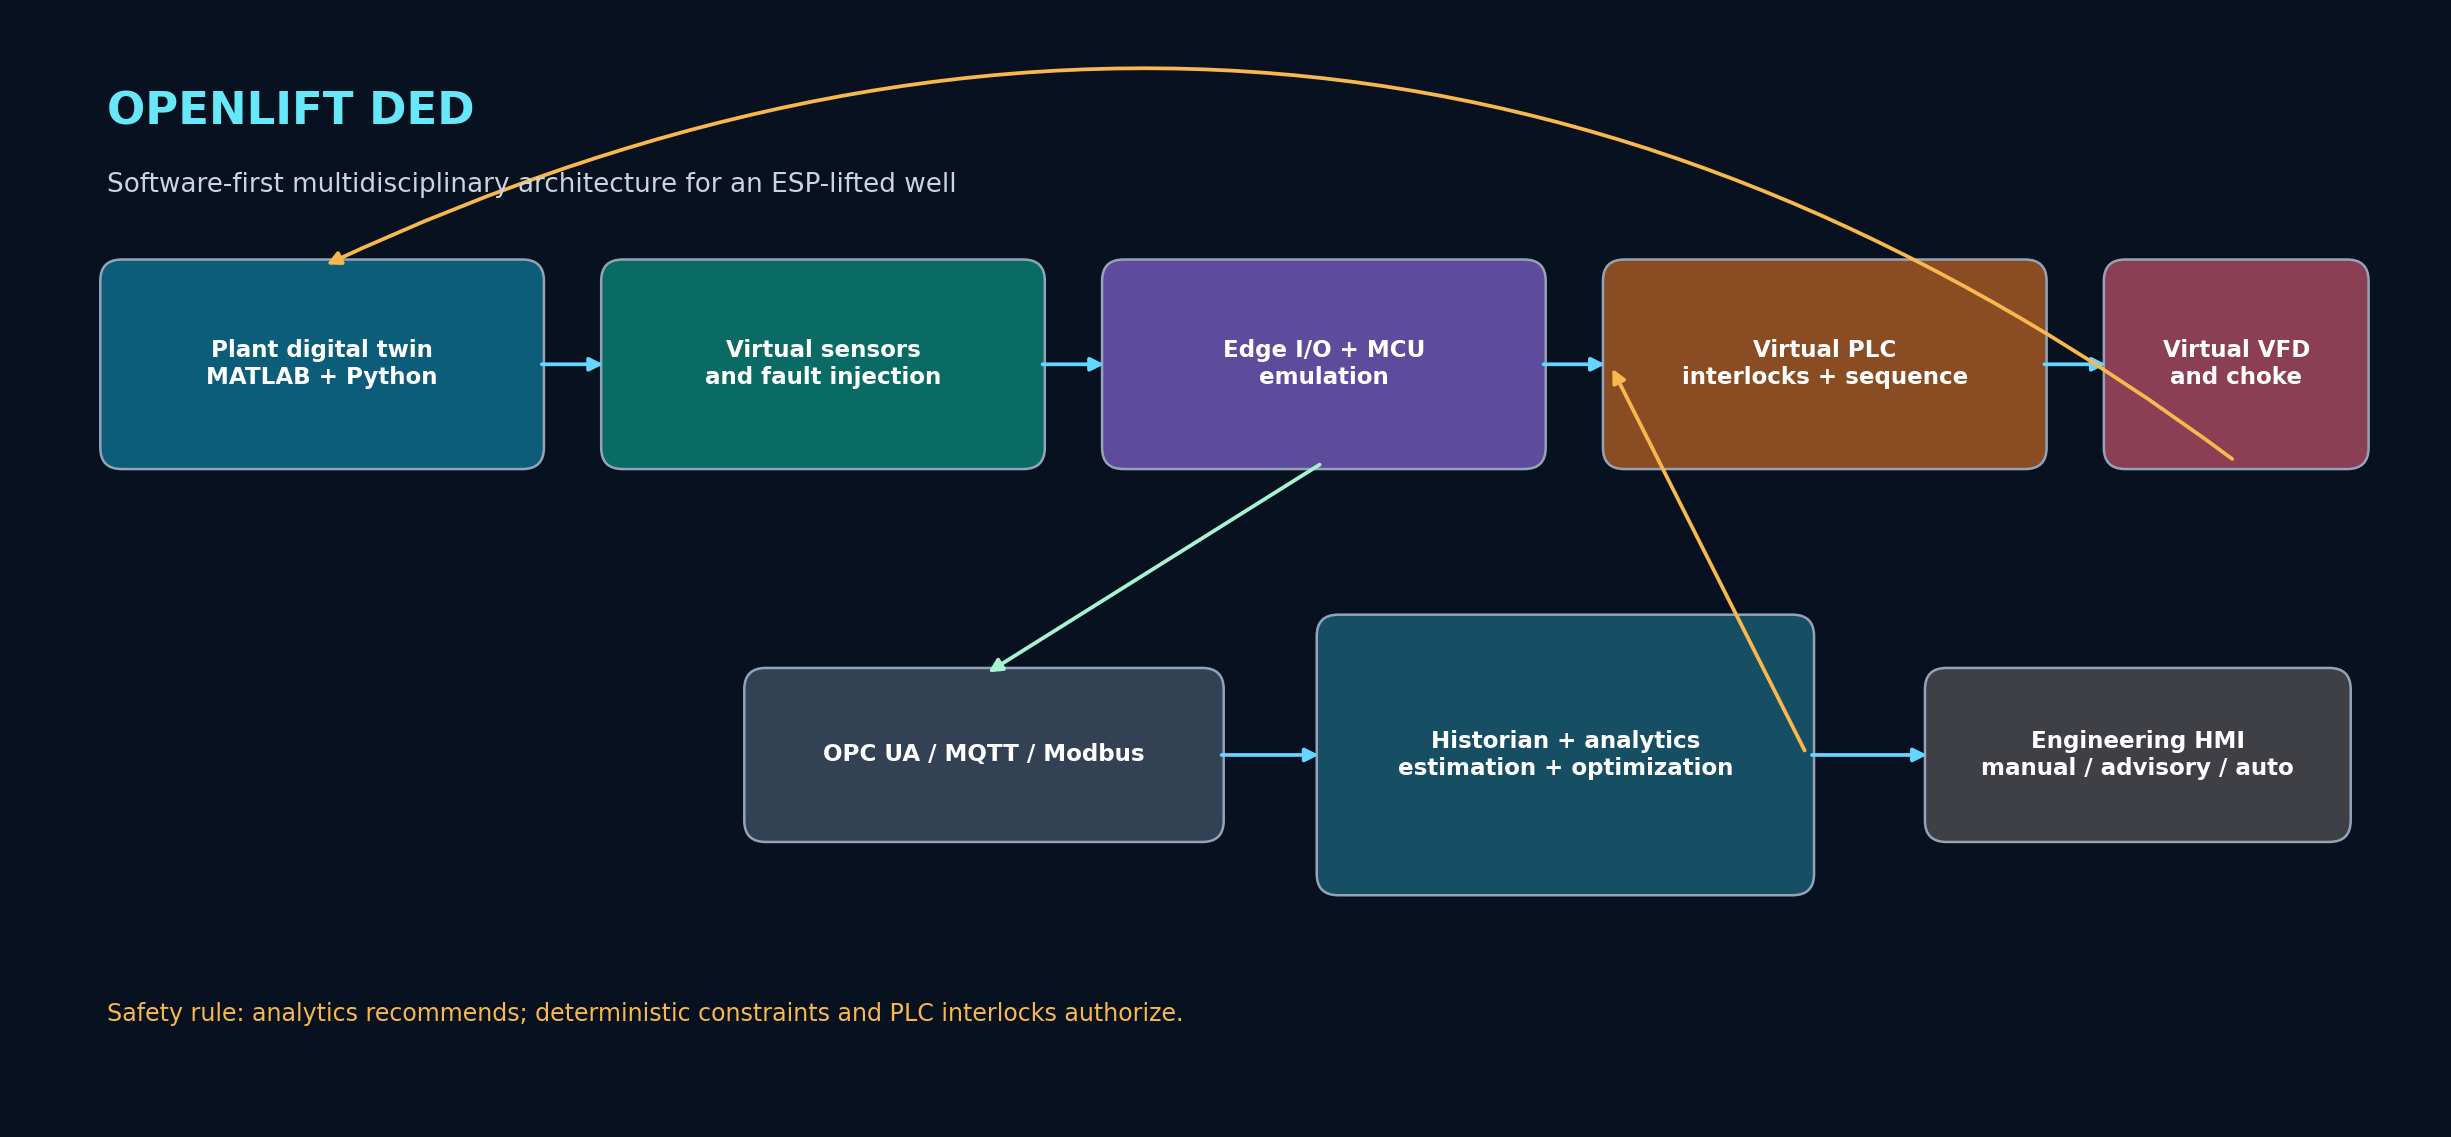
\includegraphics[width=0.94\textwidth]{../docs/assets/system-architecture.png}
\caption{OpenLift DED architecture. Analytics may recommend a command, but only deterministic constraints and PLC interlocks authorize plant actuation.}
\label{fig:architecture}
\end{figure*}

OPC UA, MQTT, and Modbus interfaces connect the controller, historian, analytics, and HMI. The analytics layer contains a state estimator, virtual flow meter, anomaly detector, health model, optimizer, uncertainty output, and out-of-distribution checks. The HMI provides manual, advisory, automatic, degraded, trip, fault-injection, and replay modes. OpenPLC provides an accessible IEC 61131-3-compatible route for the virtual controller \cite{openplc}, while FUXA supports an open web HMI route across common industrial protocols \cite{fuxa}.

The electrical work package defines conceptual power and control paths, protection assumptions, load and cable schedules, terminals, I/O, and earthing. The PCB work package specifies isolated 4--20 mA and 0--10 V inputs, 24 V digital interfaces, protected outputs, RS-485, watchdog, and diagnostic functions. FreeCAD and KiCad enable open, reviewable mechanical and electronic design artifacts \cite{freecad,kicad}. These digital artifacts are verified for interfaces, ERC/DRC findings, and collisions; no hazardous-area or field compliance is claimed.

\section{Mathematical Formulation}
The initial reservoir inflow model is
\begin{equation}
q=J(P_r-P_i),
\label{eq:ipr}
\end{equation}
where $q$ is liquid rate, $J$ is productivity index, $P_r$ is reservoir pressure, and $P_i$ is pump intake pressure. A later implementation may replace (\ref{eq:ipr}) with a calibrated nonlinear inflow relationship.

Pump head uses a nominal curve and affinity-law scaling:
\begin{equation}
H(q,N)=H_0\left(\frac{N}{N_0}\right)^2
-k_q\left(\frac{q}{N/N_0}\right)^2,
\label{eq:pump}
\end{equation}
where $N$ denotes speed or VFD-frequency equivalent. The system pressure includes hydrostatic, wellhead, tubing, and choke contributions. Hydraulic power is $P_h=q\Delta P$ after unit conversion, and electrical power is $P_e=P_h/(\eta_p\eta_m)$.

The state estimator will be evaluated with extended and unscented Kalman filters. A physics-residual feature is
\begin{equation}
r_k=y_k-\hat{y}^{\mathrm{physics}}_k,
\label{eq:residual}
\end{equation}
which allows the health model to compare observed behavior with the model prediction without mislabelling ordinary physical variables as a physics-informed neural network.

The constrained controller minimizes
\begin{equation}
\begin{split}
J_c=\sum_{k=0}^{N_p} & w_p(P_{i,k}-P_{sp})^2+w_q(q_k-q_{sp})^2 \\
& +w_E P_{e,k}+w_u\|\Delta u_k\|^2+w_s\epsilon_k^2,
\end{split}
\label{eq:mpc}
\end{equation}
for $u=[N,z_c]^T$, where $z_c$ is choke position and $\epsilon$ is a penalized slack. Hard constraints bound frequency, ramp, intake pressure, current, temperature, pump flow envelope, choke position, and solver time. A health-aware extension derates the upper speed limit as calibrated risk increases, but hard trips remain independent.

\section{Methodology}
\subsection{Engineering Design and Implementation}
The work begins with a project charter, basis of design, system requirements, tag register, assumptions, and acceptance criteria. Process, instrumentation, electrical, mechanical, PCB, embedded, PLC, HMI, MATLAB, and Python packages are then developed against those interfaces. Every requirement receives a stable identifier and verification method.

The Python implementation is the open reference plant and experiment runner. MATLAB/Simulink provides an independent equation and controller cross-check and can generate fault data, an established digital-twin use case in predictive maintenance \cite{mathworks-pump}. The PLC executes safety and sequence logic rather than machine learning. The MCU emulator performs acquisition and communication behavior. Generated evidence remains separate from configuration and source code.

\subsection{Scenario and Data Design}
The synthetic campaign varies reservoir pressure, water-cut equivalent properties, viscosity, frequency, choke, blockage, gas interference, pump efficiency, sensor faults, communication delay, and actuator response. Hydraulic states are sampled at 1--10 Hz, control and electrical variables at 10--100 Hz when needed, vibration at its native high rate, and health outputs at 0.1--1 Hz. A single sampling rate is not imposed across all signals.

External analytics use ESPset for vibration diagnosis and Petrobras 3W for well-event detection \cite{varejao2024,vargas2026}. Data splits are defined by equipment, acquisition group, simulated well, or scenario campaign rather than random time rows. Test sets include unseen operating envelope, unseen fault severity, and noisy deployment conditions.

\subsection{Verification Stages}
Stage 1 verifies each unit model using conservation checks, limiting conditions, monotonicity, affinity-law consistency, and sensitivity. Stage 2 performs open-loop sweeps. Stage 3 compares fixed speed, PID, and constrained control in model-in-the-loop and software-in-the-loop tests. Stage 4 injects randomized faults with increasing severity. Stage 5 runs the plant and virtual PLC as separate processes for controller-in-the-loop commissioning. An emulated MCU adds register and communication tests. True HIL is deferred until physical hardware is introduced.

\section{Evaluation Plan}
Table~\ref{tab:criteria} defines initial design targets. They are acceptance criteria, not reported industrial performance.

\begin{table}[t]
\caption{Planned Acceptance Criteria}
\label{tab:criteria}
\centering
\footnotesize
\begin{tabular}{p{0.48\columnwidth}p{0.39\columnwidth}}
\toprule
Measure & Initial criterion \\
\midrule
Requirements traceability & 100\% with verification method \\
Critical PLC interlocks & 100\% test pass \\
Hard-constraint violations & Zero in reference campaign \\
Normalized intake-pressure RMSE & Less than 5\% target range \\
Production tracking error & Less than 5--10\% \\
Selected-scenario energy change & More than 5\% improvement \\
MPC deadline misses & Zero; P99 below interval \\
Communication failure & Automatic degraded mode \\
PCB and CAD review & No unresolved critical finding \\
Reproduction & One-command reference run \\
\bottomrule
\end{tabular}
\end{table}

Control evaluation reports normalized RMSE, integrated absolute error, settling time, overshoot, volume, energy, energy intensity, constraint margin, solver P50/P95/P99, and deadline misses. Analytics report macro-F1, precision-recall area, false alarms per operating day, expected calibration error, lead-time distribution, and performance by fault severity and operating region. Ablations compare raw sensors, physics residuals, combined inputs, single and multimodal signals, ordinary and health-aware control, and uncertainty fallback.

Statistical uncertainty is estimated across scenario seeds and parameter sets. Conclusions are limited to the simulated envelope unless independently calibrated against field or test-rig data. Vendor-reported results are retained as motivation and are never treated as project benchmarks.

\section{Work Plan and Deliverables}
Table~\ref{tab:plan} defines the proposed part-time sequence. Each phase ends with reviewable artifacts and a release gate.

\begin{table}[t]
\caption{Proposed Work Plan}
\label{tab:plan}
\centering
\footnotesize
\begin{tabular}{p{0.14\columnwidth}p{0.54\columnwidth}p{0.20\columnwidth}}
\toprule
Phase & Output & Duration \\
\midrule
0 & Requirements, literature, tags, criteria & 2 weeks \\
1 & Physics model and open-loop tests & 4 weeks \\
2 & PID, estimation and constrained control & 4 weeks \\
3 & PLC, MCU, protocols, historian and HMI & 4 weeks \\
4 & CAD, electrical and PCB design package & 4 weeks \\
5 & Health analytics and dataset evaluation & 5 weeks \\
6 & Virtual commissioning and fault campaign & 4 weeks \\
7 & Reports, video, release and archive & 3 weeks \\
\bottomrule
\end{tabular}
\end{table}

The final package includes the requirements specification; PFD/P\&ID; model derivation; validity envelope; control report; CAD, electrical and PCB packages; embedded and PLC code; HMI; data dictionary and dataset cards; model cards; fault catalogue; validation protocol; benchmark; virtual commissioning video; reproducibility guide; safety and proprietary-boundary statements; literature and patent landscape; software bill of materials; and an archived release. A DOI is added only after the repository reaches a reviewed public release.

\section{Expected Outcomes and Limitations}
The expected result is a reproducible engineering baseline that demonstrates how control, analytics, protection, and multidisciplinary interfaces can be evaluated together. It should reveal when an apparent optimization gain is offset by constraint risk, timing failure, estimator uncertainty, or domain shift. It also creates a defensible portfolio artifact because the repository distinguishes implemented evidence, planned work, and unsupported claims.

The initial plant is lumped and single-fluid-equivalent. It omits detailed multiphase flow, PVT properties, pump-stage geometry, cable and transformer dynamics, harmonics, shaft thrust, detailed vibration physics, corrosion, scale chemistry, thermal exchange, hazardous-area design, cybersecurity assurance, and certified functional safety. Public datasets do not fully represent the target single-well configuration. Consequently, the work cannot establish field readiness, commercial equivalence, or safety compliance. Those limitations are part of the research design rather than post hoc disclaimers.

\section{Conclusion}
OpenLift DED proposes a laptop-based route from ESP process physics to virtual commissioning without conflating software evidence with field validation. The central research contribution is integration under explicit safety precedence and traceable verification. By comparing controllers and analytics on identical versioned scenarios, preserving dataset groups, reporting uncertainty and timing, and publishing the entire engineering package, the project can produce useful evidence while remaining independent of proprietary vendor technology.

\IfFileExists{IEEEtran.bst}{\bibliographystyle{IEEEtran}}{\bibliographystyle{ieeetr}}
\ifofficialieee
\bibliography{references}
\else
{\footnotesize\bibliography{references}}
\fi

\end{document}
